%%%%%%%%%%%%%%%%%%%%%%%%%%%%%%%% 
\section{The Charge Readout System} 
\label{sec:detectors-fd-alt-chg-readout}

In the liquid-gas dual-phase LArTPC concept, the ionization charge is
extracted into the argon gas phase where it is amplified by a Large
Electron Multiplier (LEM) which triggers Townsend multiplication in
the high electric field regions within the LEM
holes~\cite{Bondar:2008yw}. The electrons are efficiently extracted
from the liquid with an electric field of around 2~kV/cm and amplified
with a field of about 30~kV/cm applied across both electrodes of the
LEM. The amplified charge is then collected and recorded on a
two-dimensional segmented anode. The anode consists of a set of strips
(views) that provide the $x$ and $y$ coordinates of the event with a
3.125~mm pitch. A sketch with the typical electric fields between each
stage is shown in Figure~\ref{fig:setup}. Table~\ref{tab:crp_dist}
shows the inter-stage distance and the tolerances required to get a
uniform gain within $\sim$5\%.
\begin{cdrfigure}[Dual-phase readout]{setup}{Illustration of the electric fields in the amplification region of a dual-phase LArTPC. The simulated field lines in dark blue are an  indication of those followed by the drifting charges (without diffusion).}
 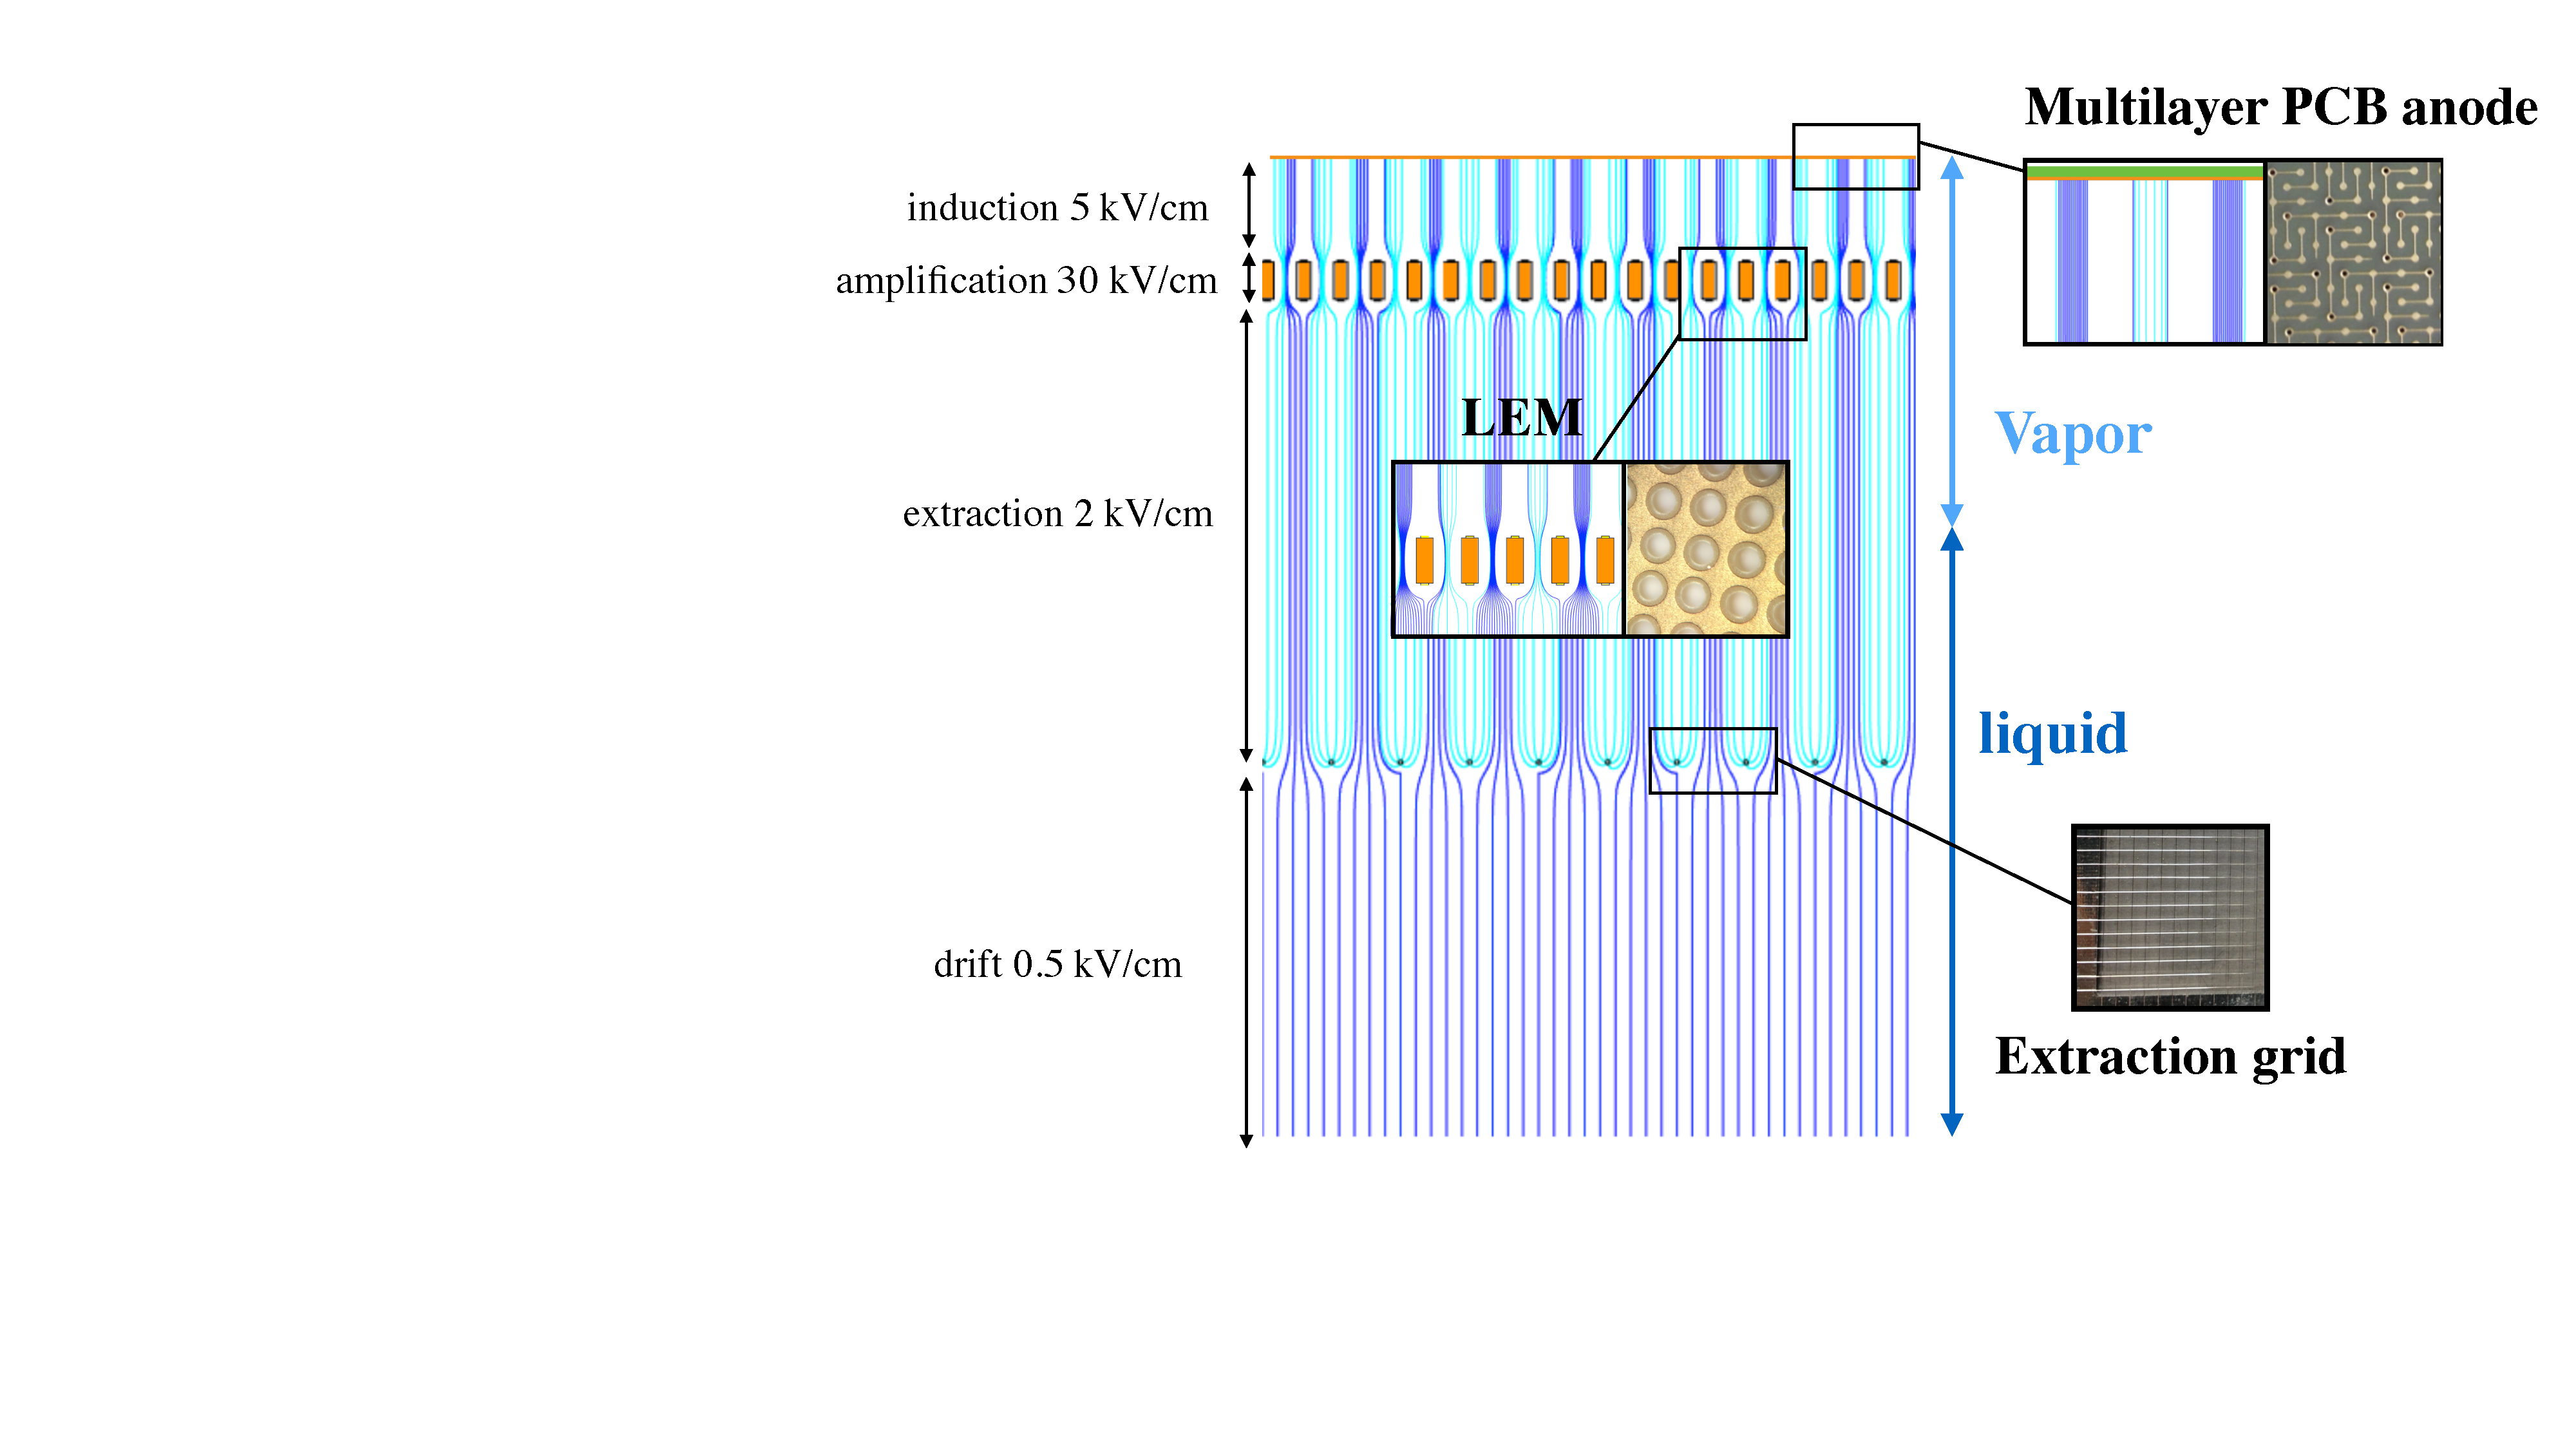
\includegraphics[width=.8\textwidth]{double_phase_principle.pdf}  
\end{cdrfigure}
\begin{cdrtable}[Interstage distances and electric field settings of the dual-phase readout components.]{lp{2cm}p{2cm}l}{crp_dist}{Interstage distances and electric field settings of the dual-phase readout components.} 
 Component & Distance [mm] & Tolerance [mm] & Electric field [kV/cm]  \\ \toprowrule
 Anode-LEM top electrode  & 2 & 0.1 & 5\\ \colhline
 LEM top-bottom electrode   & 1 & 0.01 & 30-35\\ \colhline
 LEM bottom electrode-grid        & 10 & 1 & 2 (in LAr) and 3 (in GAr)\\
 \end{cdrtable}

In the design concept of the dual-phase detector, all those stages
(extraction grid, LEM and anode) are assembled in a single Charge
Readout Plane (CRP). The CRP consists of several LEM-anode units. In
these units the 2D anodes, the LEMs and the extraction grid are
assembled together as a multi-layered sandwich unit with precisely
defined inter-stage distances and inter-alignment.
   
\subsection{The charge readout plane (CRP)}

The charge readout system of the LBNO 20~kt far detector was
modularized in units of 4$\times$4~m$^2$ CRPs. As shown in the
overview, a better matching to the DUNE cryostat geometry is possible
with an optimized 3$\times$3~m$^2$ CRP. The design and the functional
concept of the CRP are exactly the same in the two cases, however the
length of the strips is 2~m for the 4$\times$4~m$^2$ CRPs and 3~m for
the 3$\times$3~m$^2$ CRPs The following description will be based on
the LBNO CRP, as documented in the deliverables of the LAGUNA-LBNO
design study.  Each LBNO 4$\times$4~m$^2$ CRP is an independent
detector which performs the charge extraction, multiplication and
collection. The CRP is made from independent LEM and anode units of
$50\times50$ cm$^2$. The adjacent anodes can be bridged together to
form readout strips of the required length by connecting short flat
cables to KEL connectors soldered on their top side. The signals from
the last anode are brought to the front end electronics embedded
inside dedicated signal feedthrough chimneys. Each CRP is
independently hung from the vessel deck through three suspension
feedthroughs. The CRP has its own high voltage system and its
independent signal feedthroughs. A drawing of the 4$\times$4 m$^2$ CRP
is shown in Figure~\ref{fig:4_4CRP_FRONT}; some of its characteristics
are summarized in Table~\ref{tab:crp_para}.
\begin{cdrfigure}[Side and top views of the $4\times4$~m$^2$ CRP]{4_4CRP_FRONT}{Side and top views of the $4\times4$~m$^2$ CRP designed for LBNO (units in mm).}
 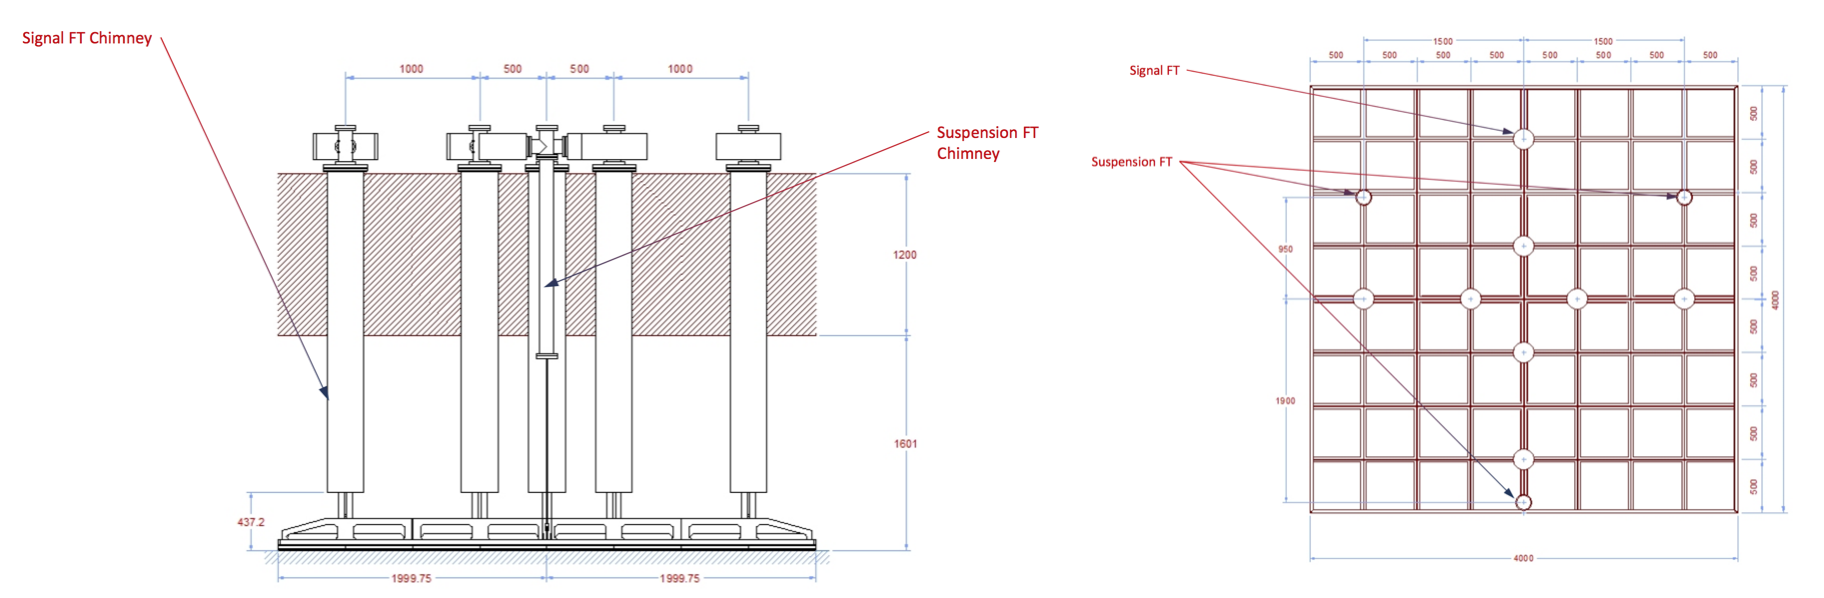
\includegraphics[width=\textwidth]{4_4_CRP_top-side-view}  
\end{cdrfigure}
\begin{cdrtable}[Numbers of components of the 4$\times$4 m$^2$ CRP]{lr}{crp_para}{Numbers of components of the 4$\times$4 m$^2$ CRP designed for LBNO} 
Component & Number \\ \toprowrule
$50\times50$ cm$^2$ anode panels & 64\\ \colhline
$50\times50$ cm$^2$ LEM  panels&  64\\ \colhline
Signal  feedthroughs & 8\\ \colhline
Suspension  feedthroughs & 3\\ \colhline
Readout strip length (m)& 2\\ \colhline
Number of channels & 5120\\
\end{cdrtable}

The entire area of the LEM and anode is active and each adjacent
$50\times50$~cm$^2$ LEM/Anode Sandwich (LAS) module has an inter-space
of only 0.5~mm. It is therefore important to note that, although
composed of independent LAS, the entire 4$\times$4~m$^2$ area of the
CRP is fully active with a small gap every 50~cm, not interfering with
the charge collection in the 3.125~mm readout pitch.

The extraction grid consists of 100~$\mu$m diameter stainless steel
wires tensioned in both $x$ and $y$ directions over the entire 4 meter
length of the CRP. They are soldered into groups of 32 on independent
wire tensioning pads spaced perpendicularly to the side of the CRP
frame. Each wire tensioning pad consists of a PCB precisely fixed on a
mechanical wire holder. The PCB hosts the high voltage connection and
has 32 soldering pads with 200~$\mu$m grooves to precisely position
the wires. During the wire soldering process each wire is tensioned by
150 g lead weights and precisely positioned inside the grooves. With
this method the precision on the wire pitch, measured under the
microscope, was better than 50~$\mu$m. The PCB is then fixed on the
wire-holder and the whole system can provide precise tension to the
group of 32 wires by pushing the holder against the CRP FR4 frame with
two stainless steel screws.

The 4$\times$4~m$^2$ LBNO CRP is integrated with feedthroughs that
serve different functionalities. The signals from the CRP are read
through 8 signal feedthroughs (SFTs) which host the front-end
electronics at its bottom and transmit the signal to the DAQ system
located on top outside of the vessel.  Each signal feed-through groups
640 channels, and the 4$\times$4~m$^2$ CRP has 5120 readout channels
in total.  The 3 suspension feedthroughs are arranged as an
equilateral triangle whose barycenter coincides with that of the
4$\times$4~m$^2$ CRP.  The suspension feedthroughs hang the CRP to the
required position and further precisely adjust the CRP level with
respect to the liquid argon surface. Figure~\ref{fig:4_4CRP_3D} shows
a 3D view of the $4\times4$~m$^2$ CRP, where the chimneys for
feedthroughs and the $4\times4$~m$^2$ stiffening frame are visible.
\begin{cdrfigure}[3D view of the $4\times4$~m$^2$ CRP.]{4_4CRP_3D}{3D view of the $4\times4$~m$^2$ LBNO CRP.}
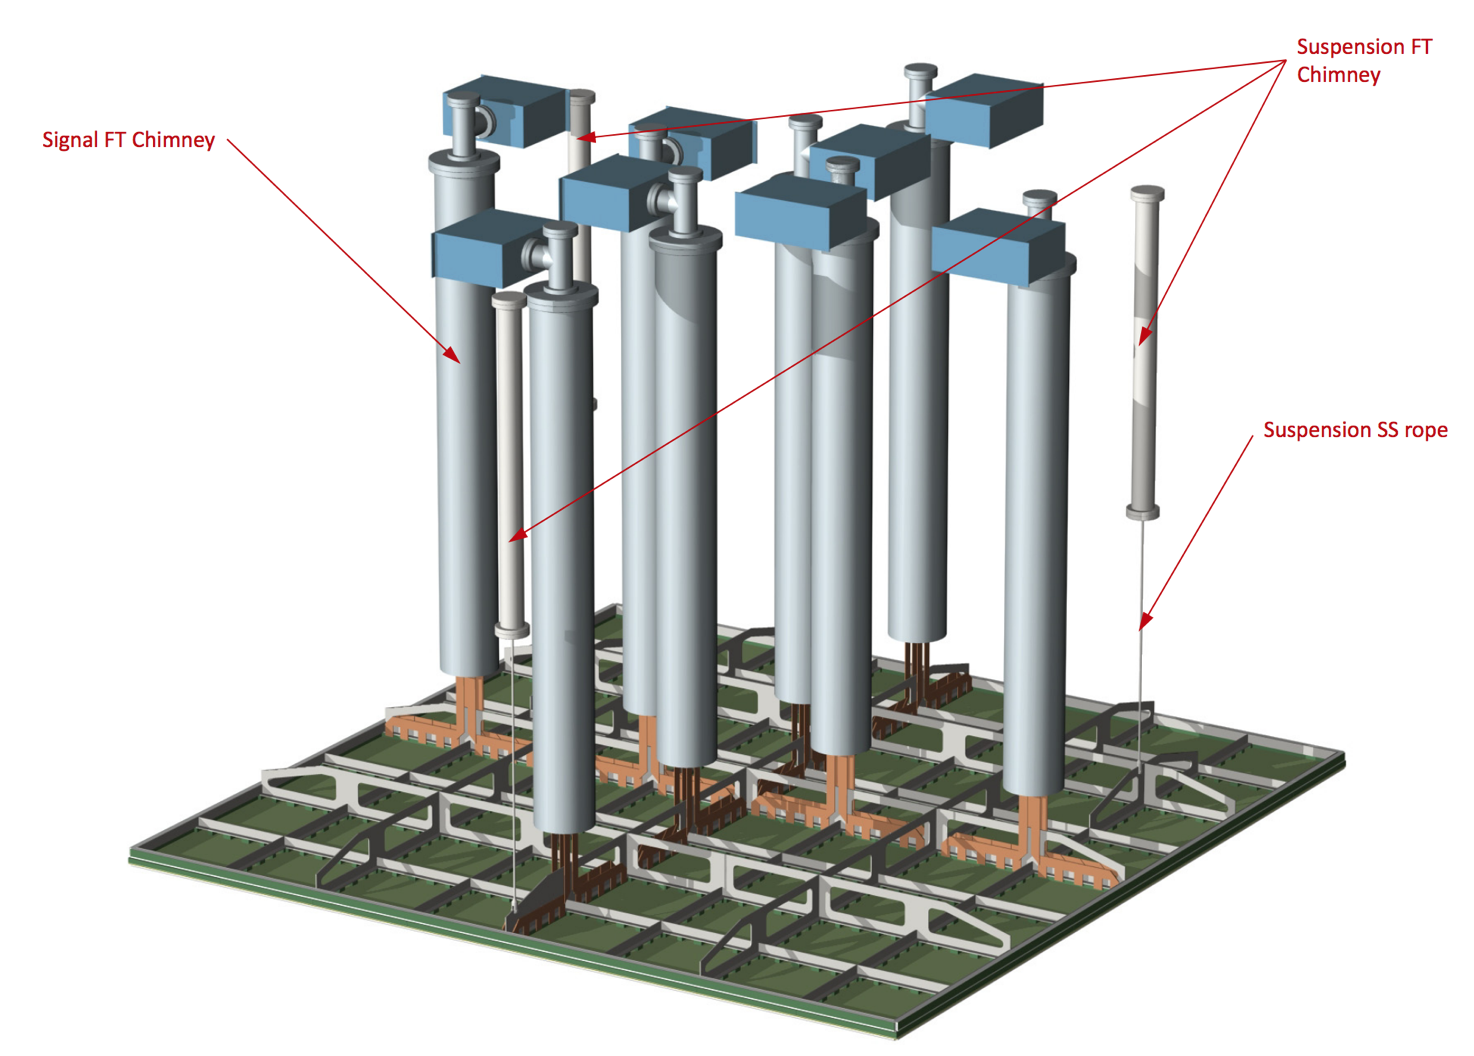
\includegraphics[width=0.8\textwidth]{4_4CRP_3D}  
\end{cdrfigure}

The DUNE CRP is a down-sized version of the LBNO one with dimensions
of $3\times3$~m$^2$ and 3 signal feedthrough chimneys and 1920 readout
channels.

\subsection{The LEM/Anode Sandwich (LAS)}

A picture of the LEMs and anodes along with a zoom on their structure
is shown in Figure~\ref{fig:LEM_anode}.
\begin{cdrfigure}[Pictures of the LEM and anode along with microscope views]
{LEM_anode}{Top: pictures of the LEM and anode along with microscope
  views. Bottom: close up of the LEM HV connectors and back view of the anode 
with the KEL signal connectors to bridge to the adjacent LAS or to connect 
flat cables going to the signal feedthrough}
 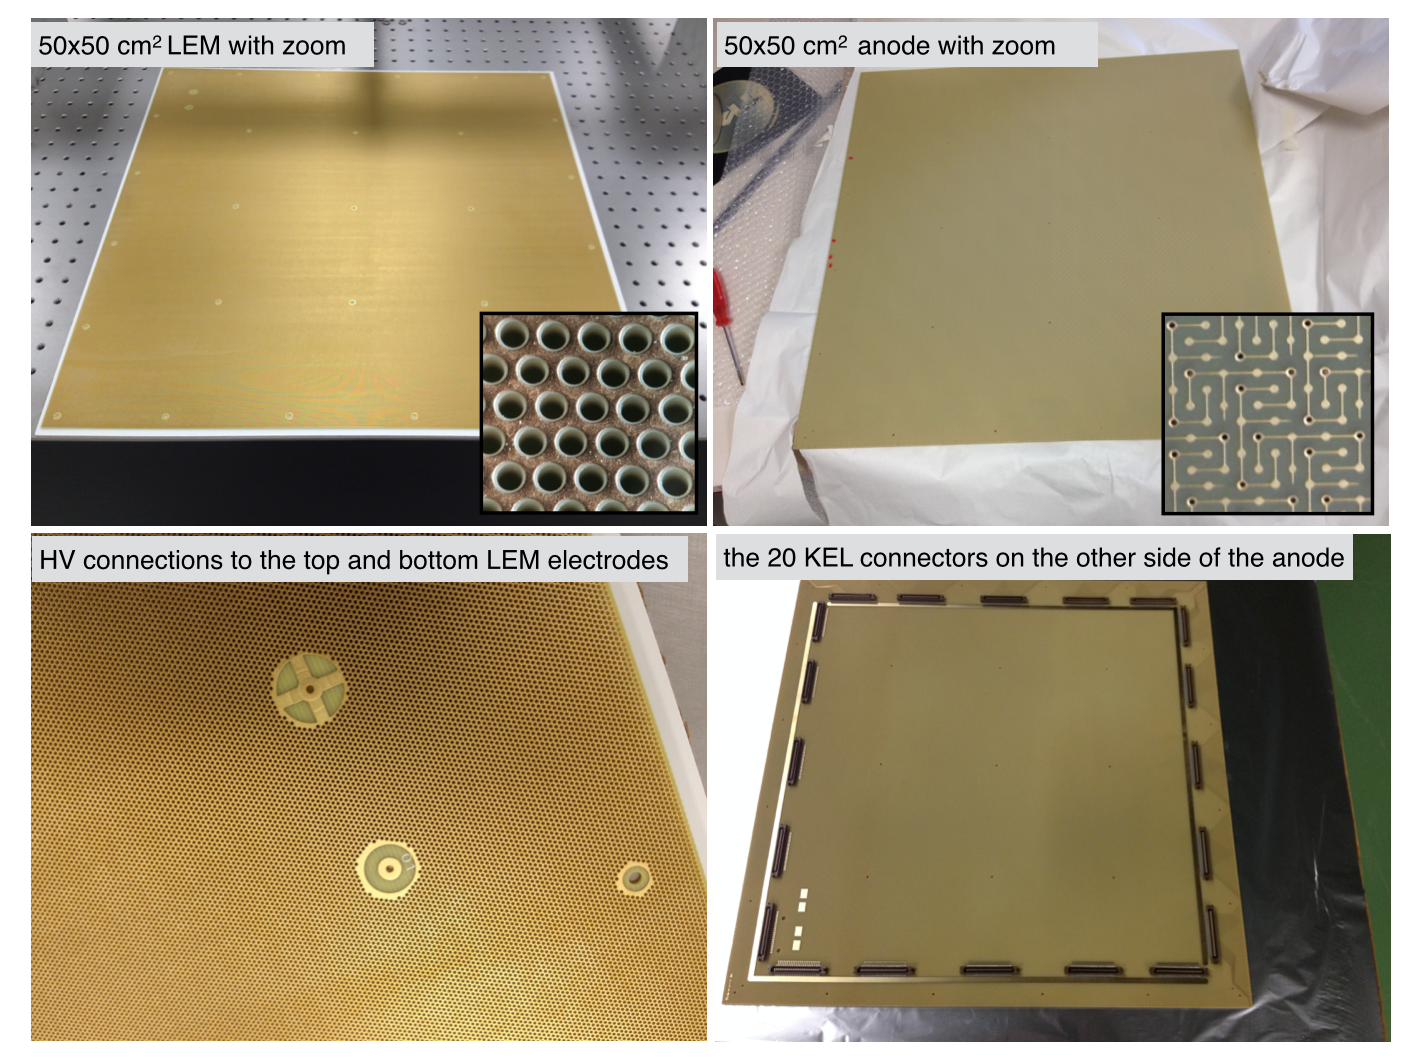
\includegraphics[width=.7\textwidth]{LEM_anode_zoom}  
 \end{cdrfigure}

The LEM and the anodes are produced by a PCB manufacturing company
called ELTOS\footnote{\url{www.eltos.it}}. Their designs are the
outcome of intensive R\&D effort of the last few years, aimed at
getting the largest signal-to-noise ratio ($S/N$) for the large area
readouts foreseen for giant dual-phase LArTPCs. They have
been, and are being, extensively studied as part of the CERN WA105
prototyping efforts (see~\ref{sec:proto-cern-double}). Below some of
the key features are summarized.

 \paragraph{The 0.5$\times$0.5~m$^2$ anode:}
The anode is manufactured from a single multilayer Printed Circuit
Board (PCB). The readout strips for both views consist of
interconnected gold plated copper tracks. The tracks pattern
corresponds to 3.125~mm readout pitch. The two views have
com-penetrating track patterns which however are electrically
insulated by ensuring the crossing connections of the tracks on the
bottom layer of the PCB with a system of vias. The design of the
patterns is such that both $x$ and $y$ views collect the same amount
of charge independently of the angle of charged particles tracks with
respect to the orientation of the readout strips. This design has been
optimized by testing various PCB layouts for the implementation of the
readout strips as described in \cite{Cantini:2013yba}.  The layout and
schematic of the anode are shown in Figure~\ref{fig:anode_sch}.
\begin{cdrfigure}[The 2D anode]{anode_sch}
{The 2D anode (left) and its schematic explaining the  interconnections 
between both views (right). One view is filled  in red and the other in white.}
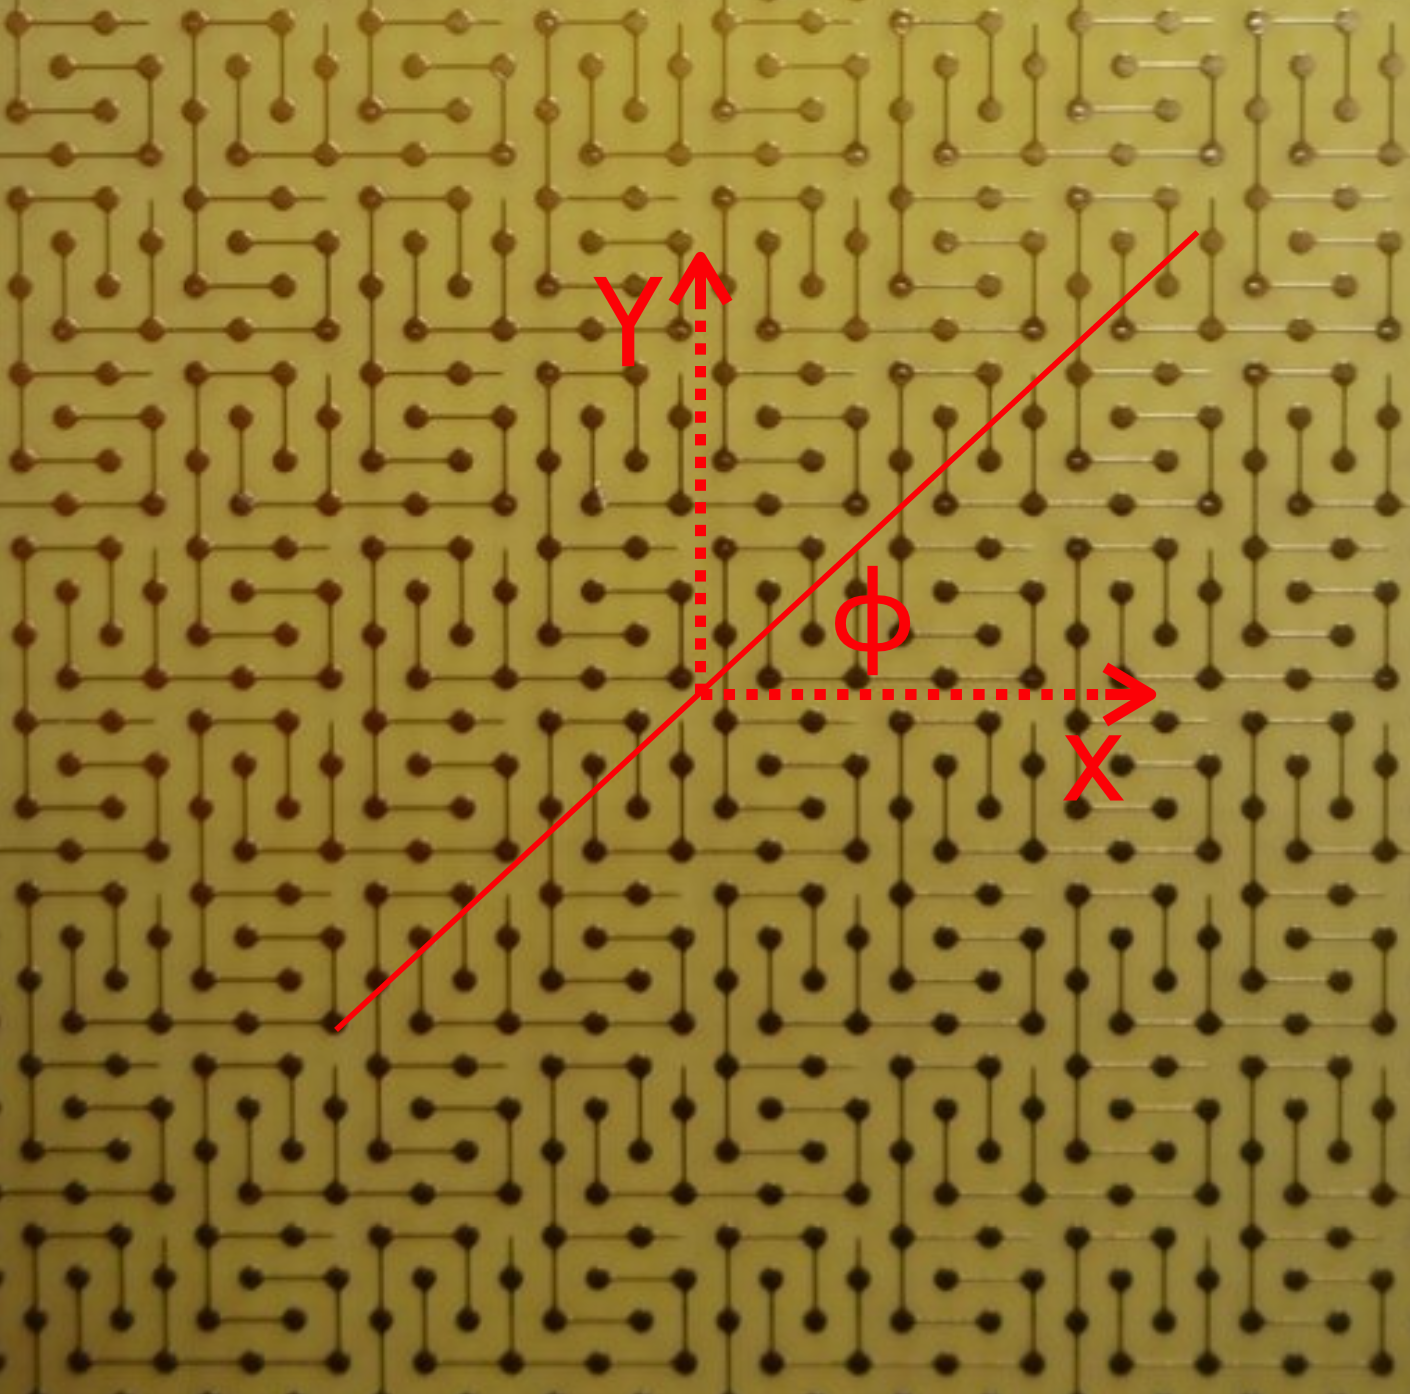
\includegraphics[scale=0.2]{anode_pcb} \hspace{0.2cm} 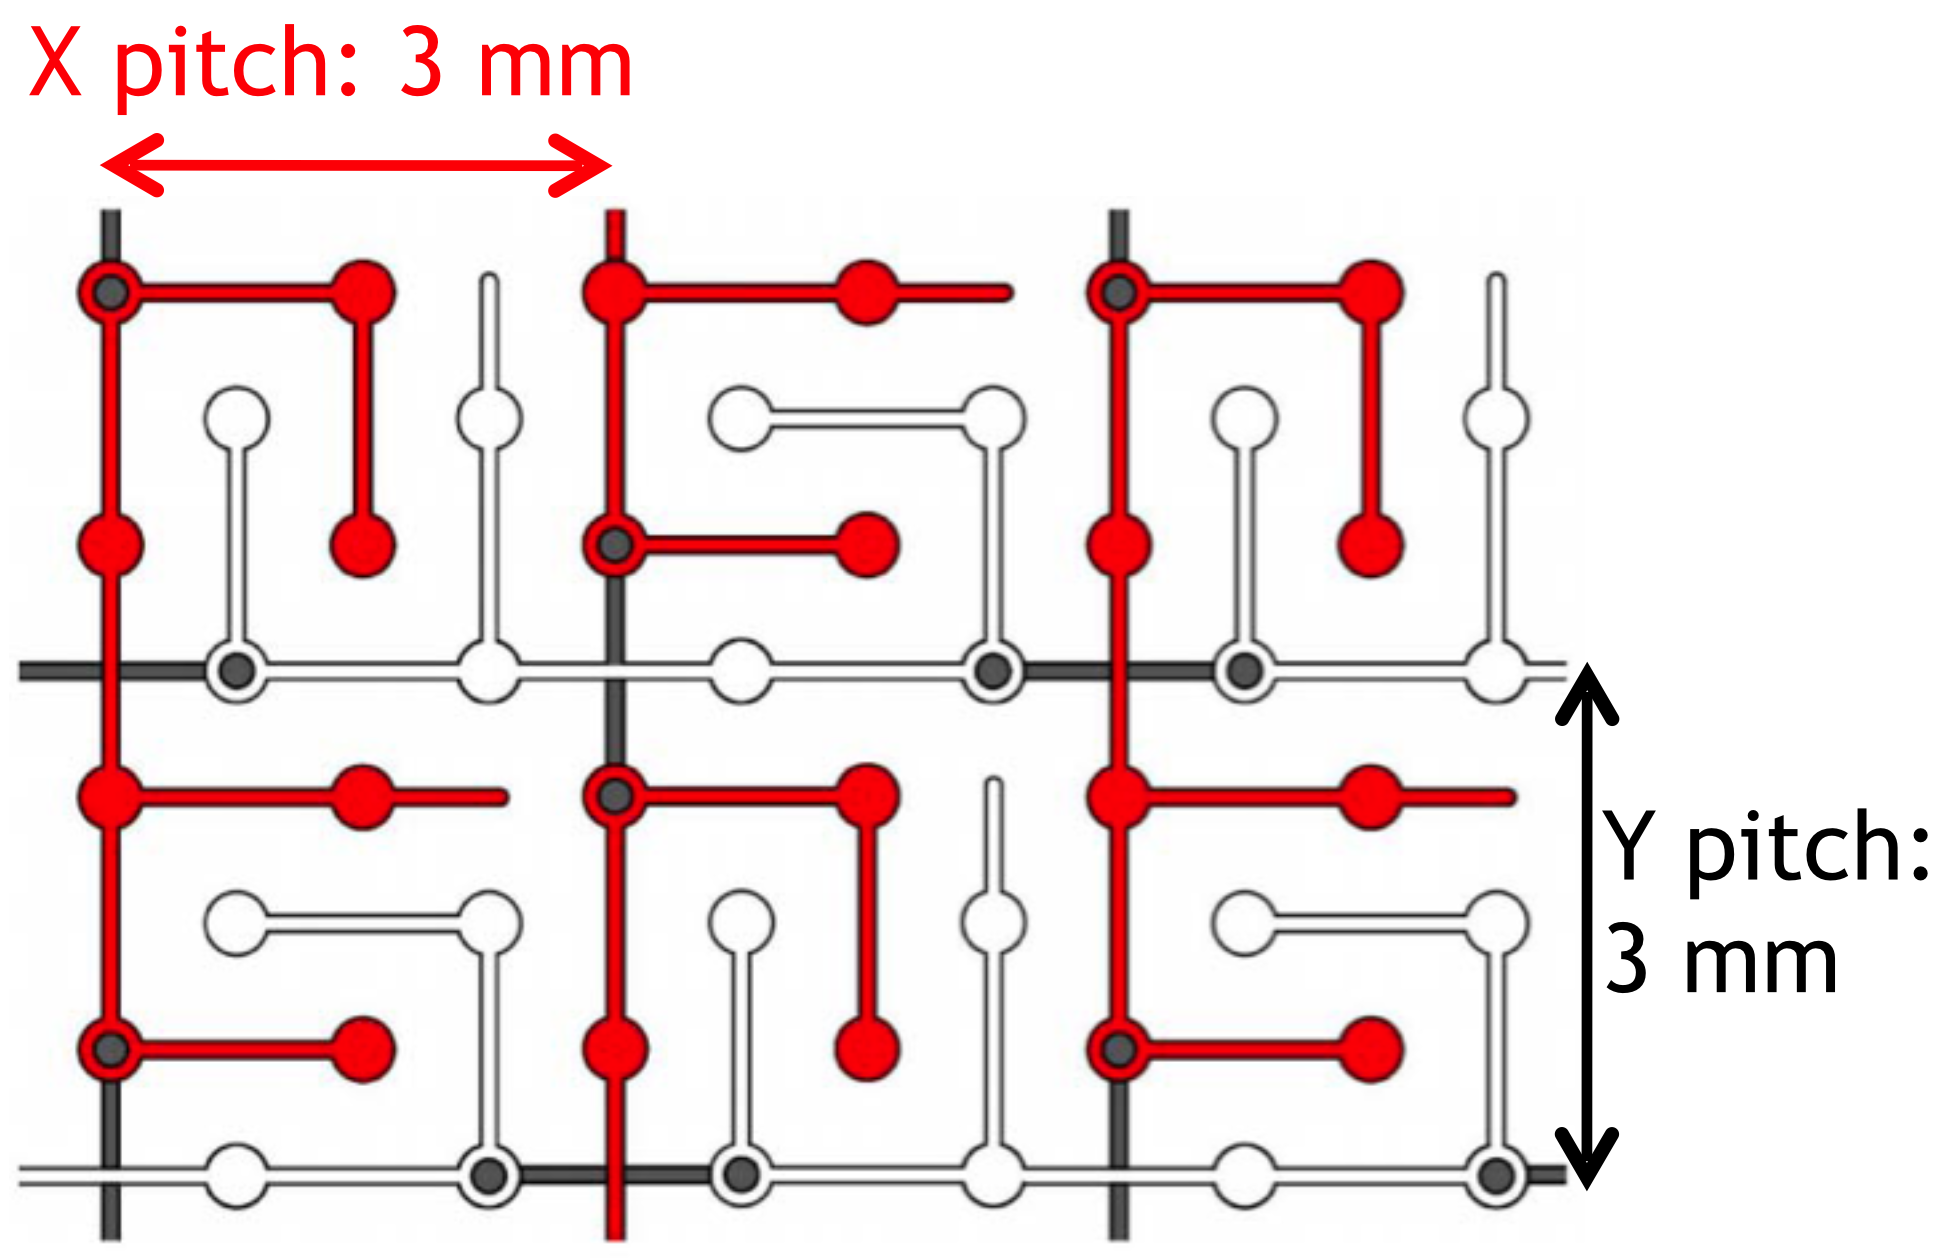
\includegraphics[scale=0.2]{anode_sch}
\end{cdrfigure}

As part of this optimization, the electrical capacitance of the
readout strips has been limited to only 150~pF/m, which translates
into an electronic noise of about $\sim$1000 electrons for 2~m readout
length.  Figure~\ref{fig:anode_res} (right) shows that the charge
sharing asymmetry between the two views is kept within 1\% . This
allows to treat the two views in a completely equivalent way from the
point of view of the reconstruction. The response in terms of the
charge collection per unit of pathlength $\Delta Q/\Delta s$ is
independent on the charged particles tracks azimuthal angle $\phi$ (see
Figure~\ref{fig:anode_res} left and middle).
\begin{cdrfigure}[Charge deposition as function of track angle ]{anode_res}
{Charge deposition per unit of pathlength measured on LEM view 0 
($\Delta Q_0/\Delta s_0$) as a function  of the track angle $\phi$ (left) and 
projection of the  $\Delta Q_0/\Delta s_0$ distribution in three $\phi$ intervals (middle). 
The right plot  shows the distribution of the difference between the total charge  collected 
on both views normalized to their sum}
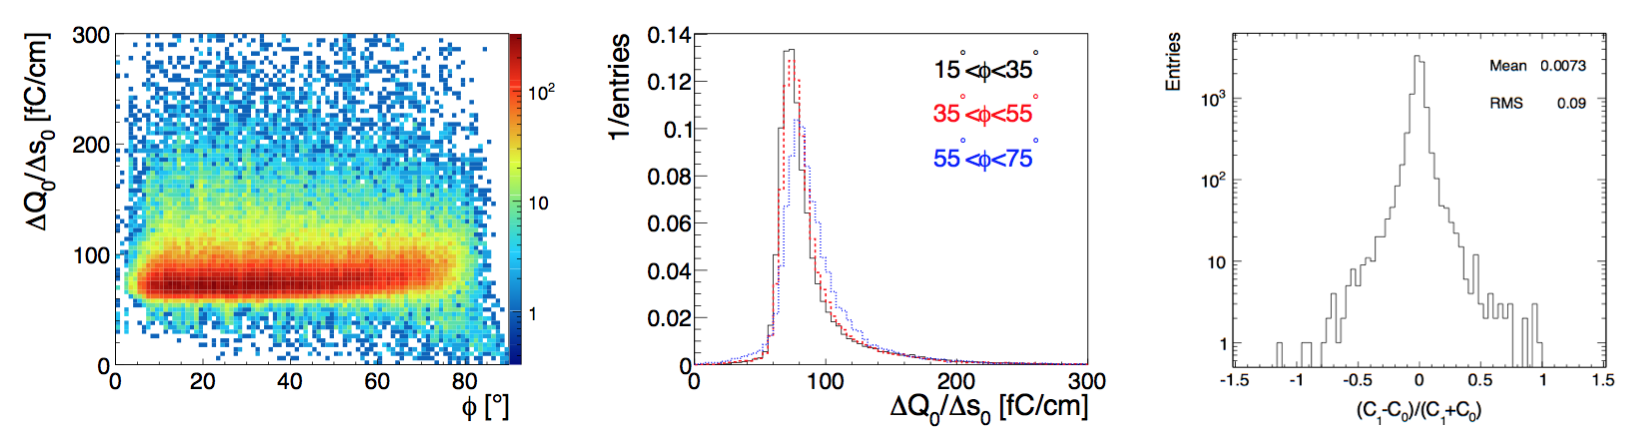
\includegraphics[width=.9\textwidth,scale=1]{anodeD_prop}
\end{cdrfigure}

\paragraph{The 0.5$\times$0.5~m$^2$ LEM:}
The LEM is built from a 1~mm tick copper-cladded epoxy PCB with
mechanically drilled holes of 500~$\mu$m diameter surrounded by a
40~$\mu$m dielectric rim around. The holes are arranged in a honeycomb
pattern with a pitch of 800~$\mu$m yielding about 200 holes per cm$^2$
and $\cal O$(500,000) holes over the entire 50$\times$50~cm$^2$
area. The holes provide the confinement of the UV photons produced
during the avalanche process and thus act as mechanical quencher to
prevent photon feedback. This property makes the LEM suitable for
operation in ultra-pure argon vapor without the addition of a
quenching gas. The amplification of the drifting charges in pure argon
vapor at 87~K with LEMs has been extensively demonstrated on a chamber
with 10$\times$10~cm$^2$ area readout (see e.g.
Refs.~\cite{Badertscher:2008rf,Badertscher:2010fi}) as well as on a
larger device consisting of a $40\times80$~cm$^2$
readout\cite{Badertscher:2013wm}.  Both setups were successfully
operated in a stable condition at constant gains of at least 15
corresponding to $S/N\approx 60$ for MIPs. Recent
studies\cite{Cantini:2014xza} characterize systematically the impact
of the rim size, insulator thickness, hole diameter and hole layout on
10$\times$10~cm$^2$ area LEMs. The response in terms of maximal
reachable gain and influence on the collected charge uniformity as
well as the long-term stability of the gain has been thoroughly
compared for these different layouts. Some results are shown in
Figure~\ref{fig:LEM}.  Gains of almost 200 could be reached and the
LEMs could be operated at stable gains of at least $\sim$15 after a
charging up period of about a day.
\begin{cdrfigure}[LEM performance vs geometry]{LEM}{Performance of the LEMs with different geometry parameters. Left: effective gain vs. LEM electric field; right: the stabilisations of the effective gain over time.}
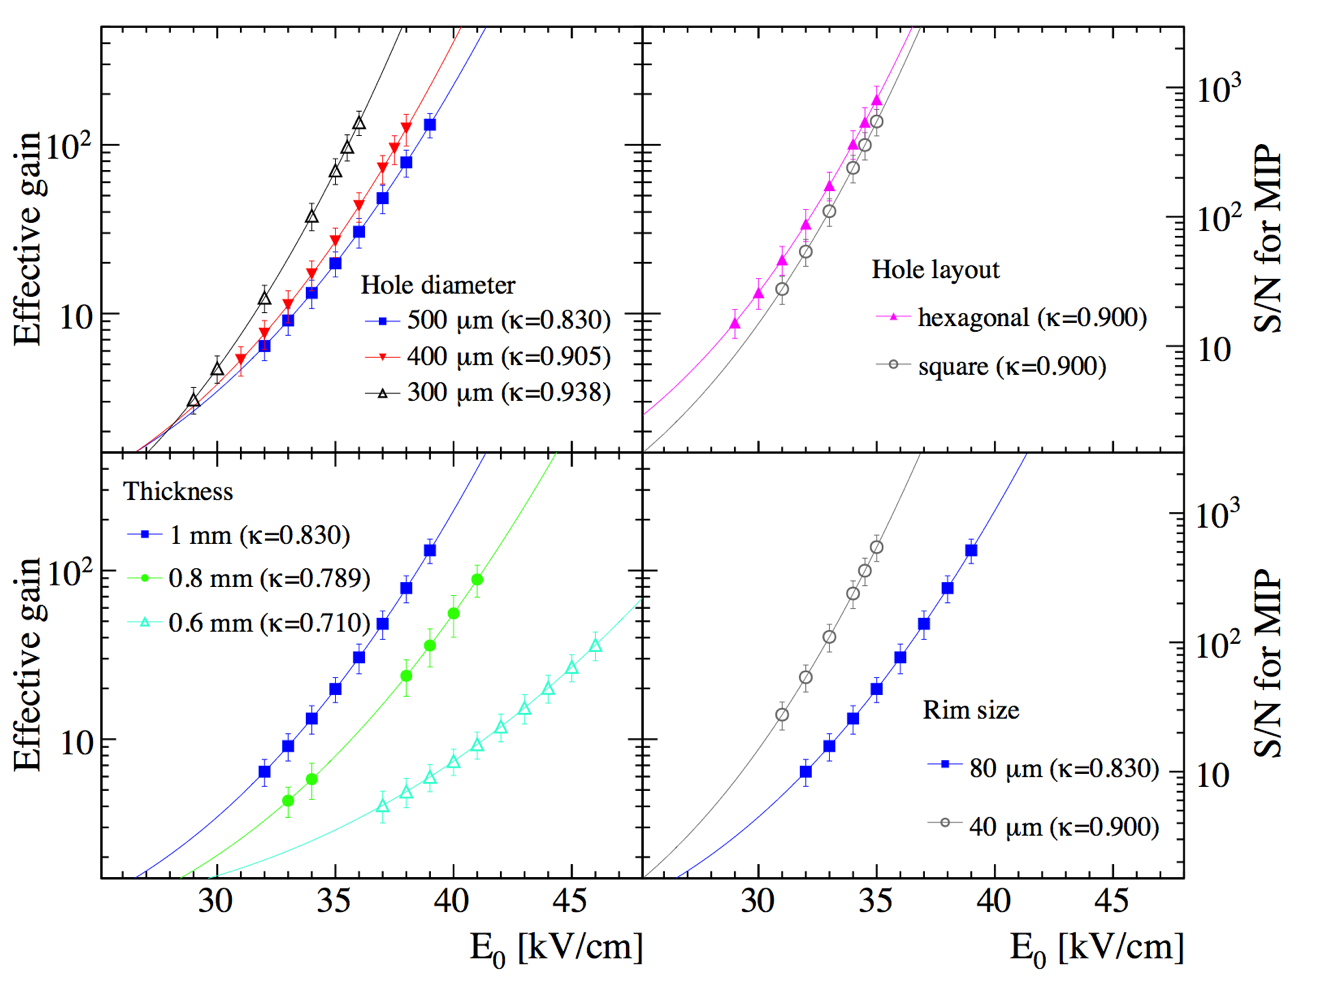
\includegraphics[scale=0.35]{4}
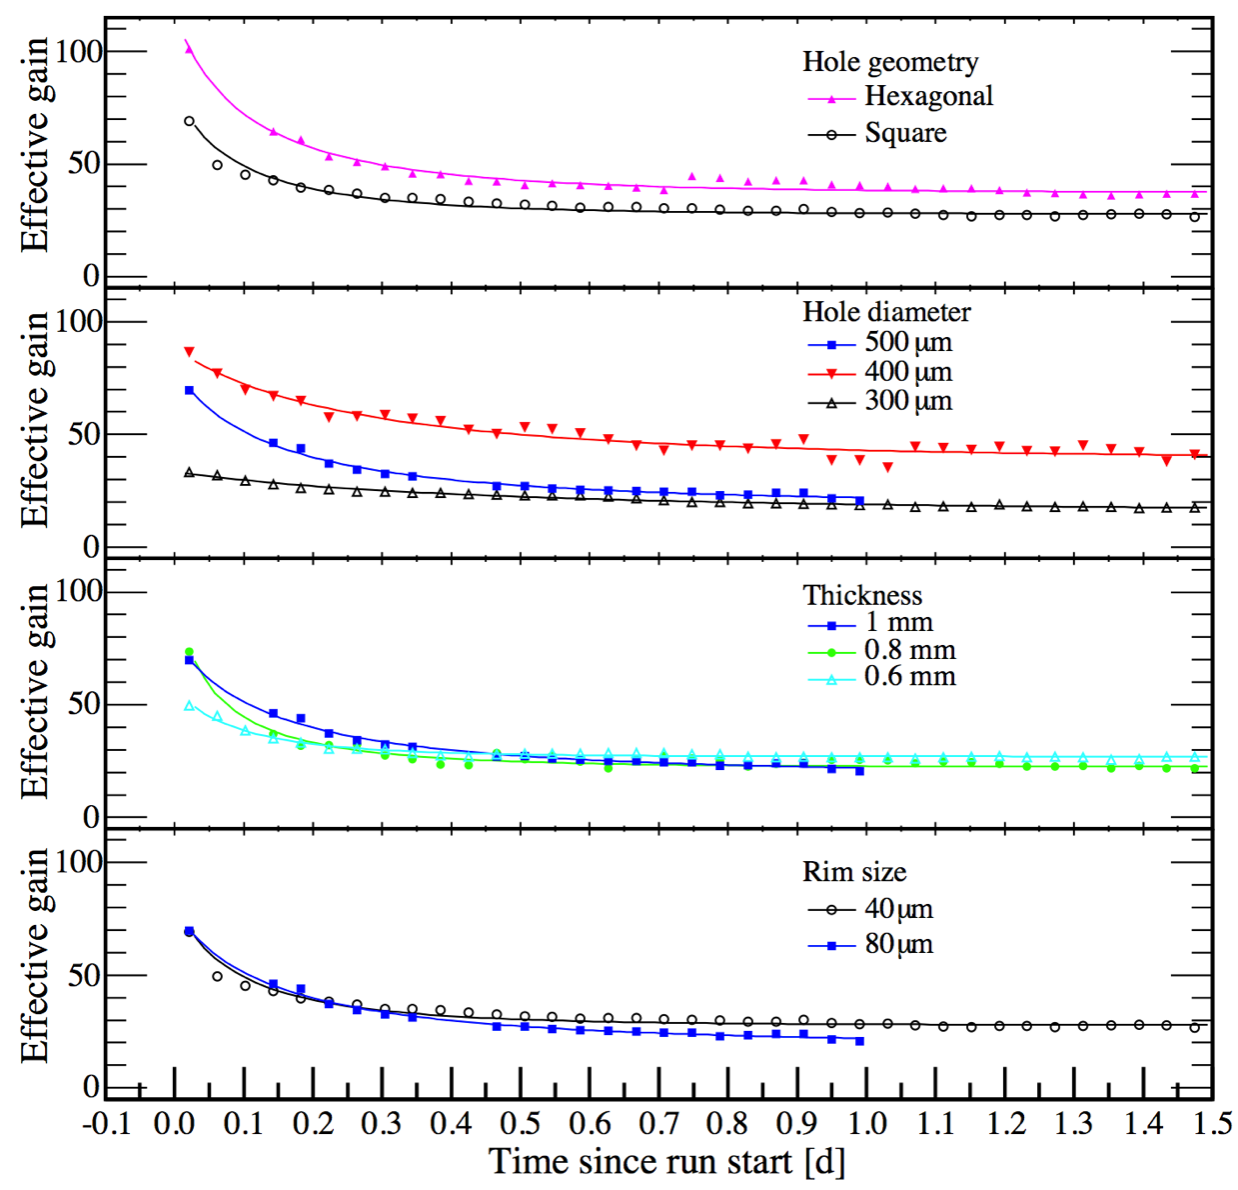
\includegraphics[scale=0.32]{3}
\end{cdrfigure}

\paragraph{LAS Assembly:}

Figure~\ref{fig:LEM_metro} shows pictures of the anode and LEM
sandwich.  They are fixed together with 29 M2 PEEK screws each
containing a precisely machined 2~mm thick pillar in order to
guarantee a constant interstage distance between the entire
$50\times50$~cm$^2$ area. The dead zones caused by the supporting
pillars and the 2 HV pins on the LEMs are minimized and correspond to
less than 0.5\% of the total area. The interstage distance between the
LEM and anode in the LAS has been measured in many points. The results
are shown in Figure~\ref{fig:LEM_metro} and are described in
\cite{EDMS_metro_lem_anode}. They indicate that the planarity is
within the required tolerance of 2~mm$\pm$100~$\mu$m .
\begin{cdrfigure}[LEM/anode sandwich metrology]{LEM_metro}{Close up pictures of the LEM/anode sandwich. The two
       bottom figures show a the measurement at the CERN metrology lab
       and a histogram illustrating the measured gap between the LEM
       and anode in various points. As can be seen the distribution is
       centered on the nominal distance of 2~mm and has an RMS of
       about 100$\mu$m.}
     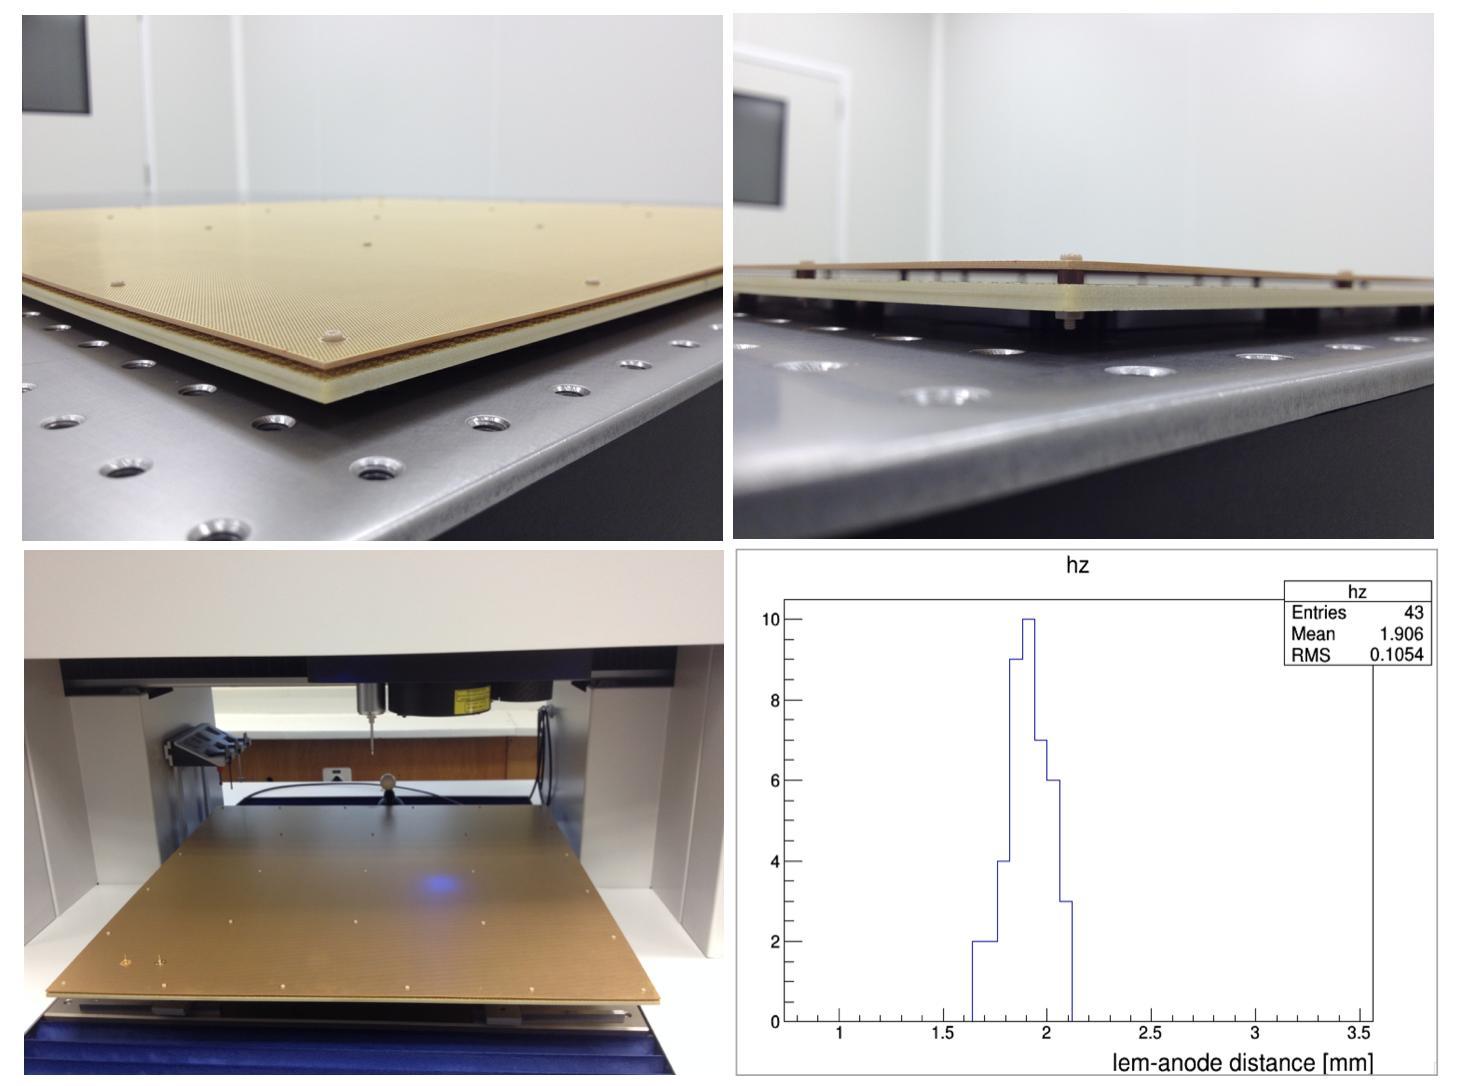
\includegraphics[width=.7\textwidth]{LEM_metro}
\end{cdrfigure}

The entire mounting sequence of the sandwich as well as that of the
different elements of the CRP are all being addressed in the WA105
prototype detectors. An example of a sandwich assembly on a
$3\times1$~m$^2$ CRP is shown in Figure~\ref{fig:CRP_assembly}.
\begin{cdrfigure}[Pictures of the assembly of a $3\times1$m$^2$ CRP.]{CRP_assembly}{Pictures of the assembly of a $3\times1$m$^2$ CRP.}
     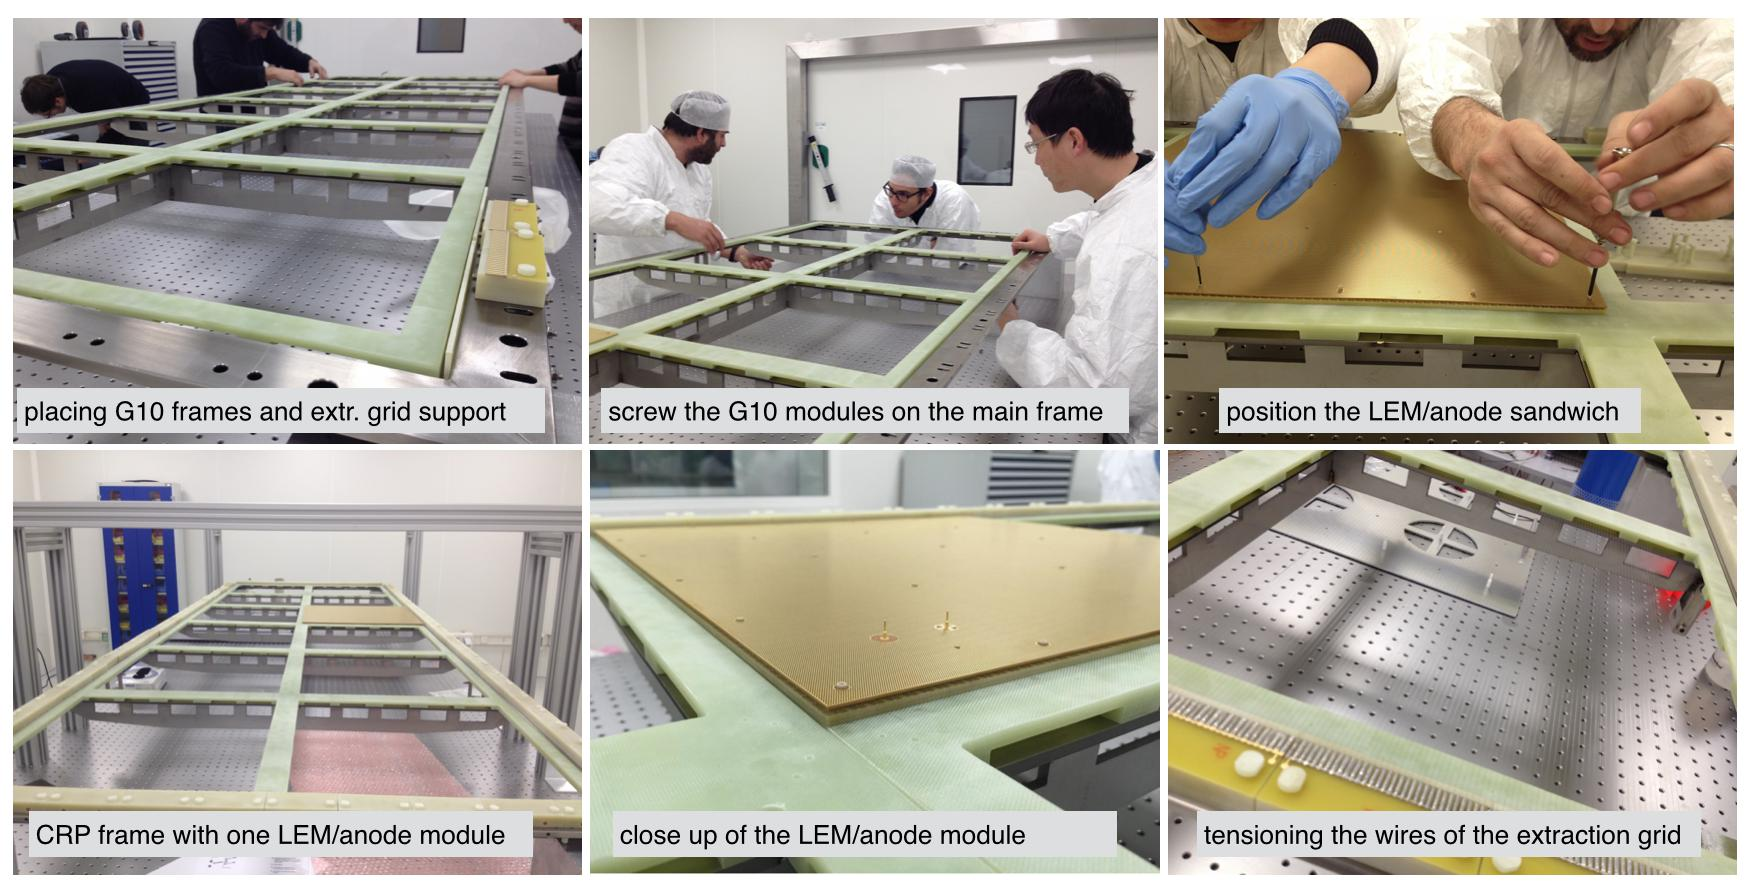
\includegraphics[width=\textwidth]{311_CRP_assembly}  
\end{cdrfigure}
